\section{Evaluation}

\begin{figure}
\centering
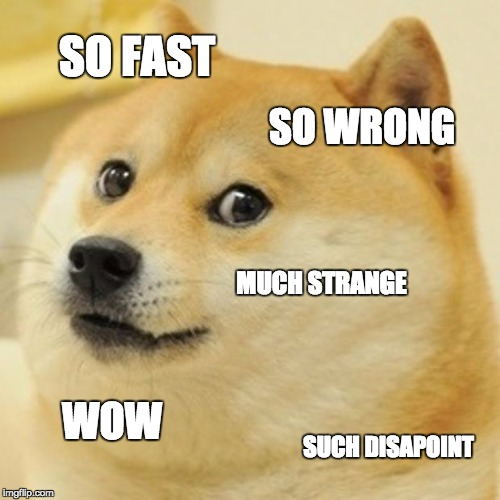
\includegraphics[width=\linewidth]{Z}
\caption{Servers are hard to get to produce reliable results.}
\end{figure}

In this section, we report on our evaluation of the practicality of
our discipline. 

\subsection{Quantitative Evaluation}

Our first evaluation is a quantitative analysis of running our tool on a
an existing repostory. In doing so we hope to answer a question:

{\bf RQ1.} Does our tool detect SemVer violations?

We know from the proof that if the interface is fully specified, we can
truthfully detect SemVer violations. The statement does contain 
inherent confounding factors, are test expressive enough to detect
violations, and are tests too strict, and would therefor over-approximate 
the interface.

The first confounding factor can easily be related to the problem of
test coverage. Test can be too specific to correctly cover all features
of the program. It is therefor reasonable to ask if an incomplete
specification still can report errors. We have decided to test our tool
on an existing library, mocha\cite{mocha}. Mocha is an testing library,
and was ideal because it had many versions, and was well tested. Mocha
contained 2 interesting test targets;``test-all'', which runs all tests
, and ``test-jsapi'' which tests an internal API\@. These tests were of
cause not designed to follow our discipline, but it enable to answer if
we are able to find any violations at all, assuming that they were. We
ran the tool for each release in the library and collect the breaking
change and added feature violations for each release. For each version
we report the number violated tests, If one test is in multiple versions
it might be counted multiple times, but that also emphasises the
importance of the test, since it survived for multiple releases.

The second confounding factor, whether too many violations would be
reported, is the most controversial. Many developers has claimed that
merely adhering to SemVer given their internal definition of the
interface would force them to bump the mayor version every
update\cite{backbone-2888,exoplayer-1382,crawford-not-semver}. This problem could be
more pronounced, if the interface was clearly specified using tests, and
SemVer was checked with a non-compromising tool. To address this factor,
we have simulate running the bump tool for each release in the history
of the mocha tool. The new version history is then be a worst-case
scenario, where the developers did not expect their tests to describe
the interface and was not warned about violations before releasing.

Lastly we did some background analysis on the framework to better
understand the composition of the library. To do this we did a
cumulation of names of tests violations and compared it to the
cumulative test names of each version.  That enables us to detect the
density of the violations in the library. This density is interesting
when making conclusions about the two factors, and will help us better
make determine whether the findings of this library applies to other 
libraries.

\subsection{User Study Evaluation}
Our second evaluation is a user study of the efficacy of our
approach. We focus on 

{\bf RQ2.} Without any assumptions about the test suite, does our tool
detect SemVer violations?

{\bf RQ3.} How difficult is it to adopt our discipline of writing API
tests?

To answer {\bf RQ2}, we manually inspected the {\em possible\/} SemVer
violations reported by our tool, in order to determine whether any of
them represent true violations. In particular, we ask whether the test
failure was due to an illegal change in the interface (in which case
the failure is a true violation), due to non-adherence to our
discipline, or for some other reason.

While reviewing the violations for {\bf RQ2}, we refactored failing
tests to adhere to our discipline whenever possible. To answer {\bf
  RQ3}, we recorded the time required for the refactoring. We also
looked for any inherent limitations of our approach that may make
adherence more difficult.

This study was conducted by the authors, who had no prior knowledge of
the internals of Mocha. Lacking ground truth for what the ``true''
interface is, we consulted the Mocha documentation, source code and
comments, and version history to make the best determination
possible. Whenever multiple interpretations were possible, we gave
Mocha developers the benefit of the doubt, choosing the interpretation
that would minimize SemVer violations.

\marktodo{Hey guys should we move this to our approach? Maybe, hey?}{I
  think maybe, sure.}
\subsection{Violation Density Hypothesis}
We hypothesize that the density of violations, defined as the average
number of violations per test, will be lower when cross-verstion
testing the {\tt test-jsapi} suite than when cross-version testing the
{\tt test-all} suite. We expect this to be true because even though
the mocha developers don't follow our testing discipline, they do
follow SemVer and identify the {\tt test-jsapi} test suite as their
interface tests. Therefore, we expect {\tt test-jsapi} to be more
consistent across versions than average. If the density of violations
is much lower for {\tt test-jsapi} than for {\tt test-all}, it will
give us some confidence that {\tt test-jsapi} is useful as a SemVer
specification.

We evaluated the violation density hypothesis by computing the
percentage of test cases that failed during cross-version testing of
each of the two test suites, {\tt test-jsapi} and {\tt test-all}.  We
identify several confounding factors with this approach:
\begin{itemize}
\item Manual inspection showed that {\tt test-jsapi} contains unit
  (secret) tests. There may be others, since we only inspected failing
  test cases of the version 1.0.0 {\tt test-jsapi} suite. This could
  skew the results. Still, our density hypothesis should be robust
  against this, since the hypothesis is that there are fewer secret
  tests in {\tt test-jsapi} than average, not that there are {\em no}
  secret tests in {\tt test-jsapi}.
\item Cross-version testing with {\tt test-all} sometimes crashes, so
  not all tests are run. This means we may be measuring too few
  failing in {\tt test-all} tests, which can skew the average {\tt
    test-all} failures downward.
\item Early versions of mocha depend on an old (incompatible) version
  of node.js. The incompatibility means that we cannot run {\tt
    test-all} at all for these versions, though {\tt test-jsapi} still
  works. In these cases, we under-count the number of cross-version
  {\tt test-all} tests that should be run for a version. In extreme
  cases, fewer {\tt test-all} tests are run than {\tt test-jsapi}
  tests, though {\tt test-all} by definition includes {\tt
    test-jsapi}. This can skew the average {\tt test-jsapi} failures
  upward, so we filter such cases out.
\end{itemize}

Despite these confounding factors, we found that {\tt test-all}
contains 46\% more failures than {\tt test-jsapi}, which indicates
that even though mocha developers do not follow our discipline, the
{\tt test-jsapi} is {\em more} compliant with our discipline than all
tests, indicating that there is some validity in using it as an
interface specification.  Further work is required to evaluate how
effective failure density can be to bootstrap interface specs for
projects that want to adopt our discipline.
